\documentclass[11pt,a4paper]{ivoa}
\input tthdefs

\title{Group Membership Service}

\ivoagroup{Grid and Web Services}

\author{}
\author{}

\editor{Brian Major}

% \previousversion[????URL????]{????Funny Label????}
\previousversion{This is the first public release}
       

\begin{document}
\begin{abstract}

TBD

\end{abstract}


\section*{Acknowledgments}

???? Or remove the section header ????

\section*{Conformance-related definitions}

The words ``MUST'', ``SHALL'', ``SHOULD'', ``MAY'', ``RECOMMENDED'', and
``OPTIONAL'' (in upper or lower case) used in this document are to be
interpreted as described in IETF standard RFC2119 \citep{std:RFC2119}.

The \emph{Virtual Observatory (VO)} is a
general term for a collection of federated resources that can be used
to conduct astronomical research, education, and outreach.
The \href{http://www.ivoa.net}{International
Virtual Observatory Alliance (IVOA)} is a global
collaboration of separately funded projects to develop standards and
infrastructure that enable VO applications.


\section{Introduction}

Through standard IVOA protocols, many astronomy data centres and institutes offer users access to datasets (SIA \citep{std:SIAP}, Datalink \citep{std:Datalink}, etc), metadata (TAP \citep{std:TAP}) and storage (VOSpace \citep{std:VOSpace}).  In some cases this information is proprietary--it is only allowed to be accessed by certain individuals.  Due to the wide variety and inherently institute-specific set of rules that may define how the information is proprietary, it is beneficial to the owners and maintainers of the rules to have a standard way of describing who has access to what resources.  Additionally, the rules describing resource access may be determined by an entity external to the holder of these resources.  To these ends, this document sets out a standard, programatic, and interoperable method of determining whether a given user is allowed to access a given resource.

The ideas presented by GMS enable data centres to do authorization checks in an interoperable fashion.  In the context of authorization, interoperability can viewed on two levels:  interoperability amongst the cooperating services \emph{within} a data centre, and interoperability \emph{between} data centres.  Because of the orthogonal nature of authorization, these levels amount to the same problem.

Interoperability aside, GMS describes a simple, general, maintainable, and scalable approach to performing authorization, and so is a recommended architectural pattern for managing access to proprietary resources.

\subsection{Proprietary resources}

Most facilities have a period of time in which only the Principal Investigator's team has access to observation metadata and data files.  Even without a proprietary period, time is required to verify and validate observations before they can be made public.

Projects also frequently create higher level products such as catalogs and images.  When these products are stored in a data centre, they must be accessible to only those who are authorized.

Proprietary information exists.  For it to be made available in a data centre to those with authorization, a way of performing that authorization check is required.

\subsection{Role within the VO Architecture}

\begin{figure}
\centering

% Get the architecture diagram from the TCG chair
% http://wiki.ivoa.net/twiki/bin/view/IVOA/IvoaTCG
% If they give you a PDF, for now dumb it down to a png by
% convert -antialias -density 72x72 archdiag.pdf archdiag.png
% Oh -- Notes don't need this; you'd have to remove archdiag.png
% from FIGURES in the Makefile, too.

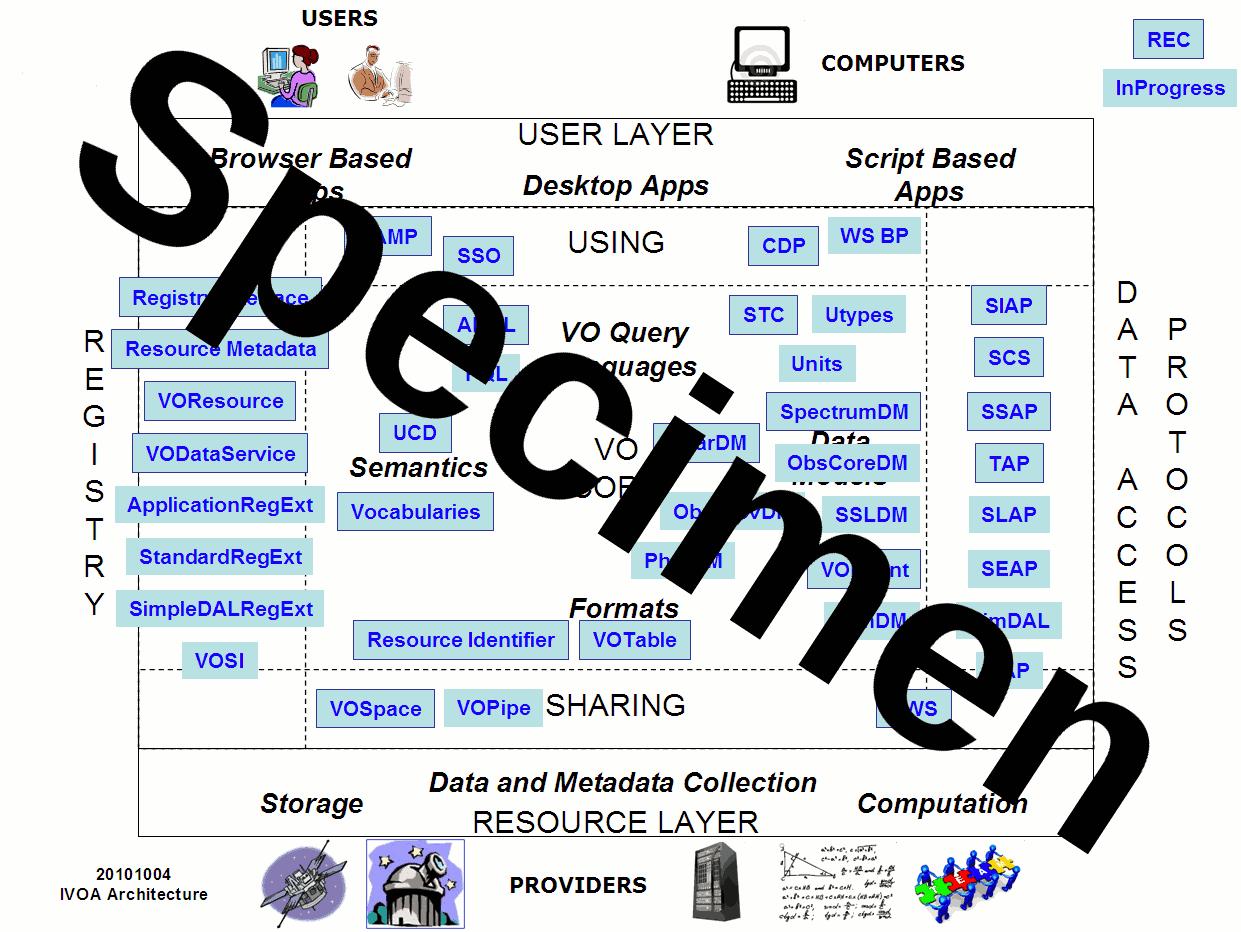
\includegraphics[width=0.9\textwidth]{archdiag.png}
\caption{Architecture diagram for this document}
\label{fig:archdiag}
\end{figure}

Fig.~\ref{fig:archdiag} shows the role this document plays within the
IVOA architecture \citep{note:VOARCH}.

\subsection{Use Cases}

\paragraph{Proprietary information} Restricting access to proprietary resources to certain users.

\paragraph{Homogeneity} Using the same mechanism to control access to proprietary resources in a data centre or in multiple data centres.

\paragraph{Scalability} A distributed mechanism that scales linearly with the resources being protected.

\paragraph{Remotely managing access} A project may wish to control access to resources that reside externally.

\paragraph{Access rule sharing} A project may consist of a variety of resources that can be all managed by the same access rules.

\paragraph{Extending the services of a data centre} A project that has hosted data and metadata at a data centre may wish to create value-added services outside of the data centre itself.  If some of the data or metadata is proprietary, the extended services may need to determine if a user is allowed to perform certain action on that data or metadata.

\paragraph{Cooperating institutes} Two or more institutes may work together on a single project that involves proprietary resources so require a common mechanism for protecting those resources.

\subsection{Definitions}

\paragraph{Authentication} User identification through credentials or identity provider.  See IVOA Single-Sign-On Profile: Authentication Mechanisms.  \citep{std:SSOAUTH}

\paragraph{Authorization} Making the decision of whether to grant a user permission to a given resource.  The decision can involve knowing the user's identity.

\paragraph{Resource} Something that may require authorization for access.  For example, a service, a data file, metadata.

\paragraph{User} An individual identified by authentication.

\paragraph{Group} A set of users who have access to a resource.

\paragraph{Grant} Giving a user authorization to access to a protected resource.

\paragraph{Revoke} Taking away from a user access to a protected resource.

\paragraph{Owner} A user or group of users who may grant or revoke access to a specific resource.

\section{Authorization Requirements}

When looking at a system that has proprietary resources that need to be protected, it is clear that there are two distinct phases to authorization:  the assignment of the rules protecting the resources, and the attempts by various users to gain access to those resources.  They are described here:

\begin{enumerate}
\item The owner(s) of a resource may, at any time, change the rules by which a resource may be accessed. This is the \emph{granting and revoking of access}.
\item When users try to access resources, the granting rules for that resource are evaluated at runtime. This is the \emph{authorization check}.
\end{enumerate}

With these phases in mind and with the use cases defined, we can state that the goals of authorization is to:

\begin{itemize}
\item To allow for restricted access certain resources: only a certain set of individuals may access certain resources.
\item To allow certain individuals to set the access rules on resources.  The owner(s) of the resources need to manage the access rules.
\item To be able to re-use granting rules between resources.  Projects must authorize access to a variety of proprietary resources.
\item To be able manage granting rules at a single location.  Projects should not have to update each resource on a change to a re-used grant.
\item To be able to reference remote granting rules.  Proprietary resources should not be confined to a single institution.
\end{itemize}

\section{Groups}

Why are groups a good model for authorization?  When a system needs to perform an \emph{authorization check} on a resource, it is trying to determine if the authenticated user is allowed access.  There are a number of options on how this can be accomplished.

A simple approach would be to add the identity of the user to the resource.  However, this is too restrictive as there may be multiple users who are allowed access.  So, we could instead add a list of user identities to the resource being protected.  This becomes a problem when there are two resources that need protecting by the same set of individuals.  This becomes difficult to maintain because a change in access rules (\emph{granting and revoking access}) would mean a change to multiple resources.

So, it becomes clear that this list of users needs to be detached and centralized so that it can be referenced and shared by multiple resources.  To do so, the list must become a single entity than can be referenced by a name.  And so, we must now have a named group of users.

But if there is a central repository of groups of users, we introduce other problems:  a single point of failure, and the inability to partition groups of users.  Thus, the \emph{location} of the group must accompany the group itself so that it is possible to have multiple collections of groups of users.

Resources must then reference a group by a URI with a location and a name that is unique within that location.  This is called the Group Identifier.

Systems must use the information in the group identifier to query location to determine if the user is a member of the group.  Because the location may be outside of the immediate vicinity of the resource, this query must be performed in a standard and accessible manner and so is defined as a RESTful interface to group membership. 

\subsection{Group Identifiers}

A Universal Group Identifier is an IVOID (\citep{std:VOID2}) used to uniquely identify groups.  For GMS, there are three important components to the group ID:

\begin{enumerate}
\item \emph{The authority} This identifies the location or instance of the group membership service.
\item \emph{The path} Always 'gms', indicating that it is a group URI.
\item \emph{The query} Identifies the group within the authority.  The name of the group.
\end{enumerate}

Below is an example group identifier:

\begin{verbatim}
ivo://authority.example.com/gms?groupName
\end{verbatim}

To resolve the host GMS service, lookup, in the Registry, the URL for resourceID:

\begin{verbatim}
ivo://authority.example.com/gms
\end{verbatim}

This may result in (for example):

\begin{verbatim}
http://server.example.com/myGMS
\end{verbatim}

This is the URL to the GMS service with information on the group named 'groupName'.



\section{Users}

The concept of users and user identity is core to group authorization.  When the owner of a resource would like to grant access to that resource to an individual, that individual must be referenced in some way.  When a system makes a call to a GMS service to determine if the user trying to access the resource is a member of a group, the GMS service needs to identify that user with the users in various groups.  

The collection of data centres and astronomy institutes likely have many ways of identifying users.  They could be using external identity providers, they could have a local database of users, or may have a combination of these and other approaches.  Section~\ref(subsection:useridentity) has some recommendations on how to best design a user identity system, but this specification does not require such a design.  Instead, it requires simply that users can be uniquely identified within the scope of a GMS service's domain.  If a user identity reaches beyond the scope of a GMS service's domain (such as an X.500 distinguished name \citep{std:RFC1779}), then it, too, may be referenced by the service.

The list of officially supported authentication protocols can be found in the IVOA Single-Sign-On Profile: Authentication Mechanisms \citep{std:SSOAUTH}.

TBD...

\section{The group management service (GMS)}

The Group Membership Service (GMS) is a RESTful API that allows for the determination of whether a user is a member of a group.

TBD...

\subsection{API definition}

Functionally required:
\begin{itemize}
\item boolean isMember(Group)
\item list<Group> getMemberships()
\end{itemize}

Group Membership System RESTful \citep{fielding00} API
\begin{verbatim}
GET /gms/groups
GET /gms/groups/{group}
\end{verbatim}

Note that there is no information about the user or the resource being protected in the GMS API.  This is intentional.
Since it is the system representing the protected resource that is making the GMS call, it already knows the context of that call.  If the ID resource were to be added to the GMS API, we would be unnecessarily coupling the resource with the data within the GMS service and creating an inflexible architecture.
The user is not a part of the API because the user is determined by identifying the authenticated caller of the service.  It must be the user (or the delegated user) making the API call as explained in \ref{section:gmsandcdp}.

\section{GMS and Credential Delegation}
\label{section:gmsandcdp}

The GMS service follows the recommendations of the IVOA credential delegation protocol \citep{std:CDP} and requires that the calls to the service to be made by the user who initiated the request.  Aside from the architectural benefits of employing this pattern, there are a number of information privacy concerns that are addressed.  User and user group membership information is private and thus should only allowed to be viewed by the users themselves.  So, the calls to GMS must be by the user, or by an authorized representative of the user.

Because it is the systems enforcing authorization on proprietary resources that need to make the calls to GMS, they must acquire the user's delegated credentials in order to make those calls.  

TBD...


\section {Implementation}

Possible ways to implement GMS

\begin{itemize}
\item Via Grouper (groups in MySQL, users in LDAP)
\item LDAP only with memberOf plugin (supports groups-of-groups)
\item VOSpace implementation: ContainerNodes = groups, DataNodes = users
\end{itemize}

\subsection{User Identity}
\label{subsection:useridentity}

TBD - describe how to support multiple identities, how to design a system where no locally stored users are needed.

\subsection{Groups of Groups}

It may be functionally attractive to support groups within groups.  If this is implemented, then the service must ensure that this representation is reflected by the service API.  For example, if an isMember(g) call is made, and the group 'g' is a group within another group in which the user is a member, then the service must return true.  Essentially, the service must denormalize (at runtime) the containment of groups within groups.

If one of the contained groups actually exists at another GMS instance, perhaps outside of the organization, then the service must transitively query that service to determine group membership.  This of course requires that the user's delegated credentials be available in the GMS service itself and within any other GMS services it may call.  Please refer to the note on the IVOA inter-service calling pattern for more detail \citep{note:IVOSvcPatterns} (not yet written!)


\subsection {Examples}

TBD

\section {Future considerations}

This document presents a standard way of making the authorization decision, but not for the granting and revoking of access.  However, a number of examples are presented on how granting and revoking can work.  These examples may define a path for standardization if the need arrises.

\appendix

\section{Convenient extensions to GMS}:

Group Management API could be provided:
\begin{itemize}
\item create/modify/delete groups
\item Add/remove members
\end{itemize}

\section{Changes from Previous Versions}

No previous versions yet.  
% these would be subsections "Changes from v. WD-..."
% Use itemize environments.


\bibliography{ivoatex/ivoabib,ivoatex/docrepo}


\end{document}
